\chapter{Индивидуальное задание}

\begin{enumerate}
	\item Неоптимизированный цикл:
	\begin{lstlisting}[language=C]
extern "C"
{
	void var003_no_pragmas(int* c, const int* a, const int* b, const int len)
	{
		int minA = a[0];
		int minB = b[0];
		for (int i = 1; i < len; i++)
		{
			if (minA > a[i])
			{
				minA = a[i];
				c[i] = minA;
			}
			else
			{
				c[i] = 0;
			}
		}
		for (int i = 1; i < len; i++)
		{
			if (minB > b[i])
			{
				minB = b[i];
				c[i] = minB;
			}
		}
	}
}
	\end{lstlisting}

	\item Конвейерная организация цикла:
	\begin{lstlisting}[language=C]
extern "C"
{
	void var003_pipelined(int* c, const int* a, const int* b, const int len)
	{
		int minA = a[0];
		int minB = b[0];
		for (int i = 1; i < len; i++)
		{
			if (minA > a[i])
			{
				minA = a[i];
				c[i] = minA;
			}
			else
			{
				c[i] = 0;
			}
		}
		for (int i = 1; i < len; i++)
		{
#pragma HLS PIPELINE
			if (minB > b[i])
			{
				minB = b[i];
				c[i] = minB;
			}
		}
	}
}
	\end{lstlisting}

	\item Частично развернутые циклы:
	\begin{lstlisting}[language=C]
extern "C"
{
	void var003_unrolled(int* c, const int* a, const int* b, const int len)
	{
		int minA = a[0];
		int minB = b[0];
		for (int i = 1; i < len; i++)
		{
#pragma HLS UNROLL factor=5
			if (minA > a[i])
			{
				minA = a[i];
				c[i] = minA;
			}
			else
			{
				c[i] = 0;
			}
		}
		for (int i = 1; i < len; i++)
		{
#pragma HLS UNROLL factor=5
			if (minB > b[i])
			{
				minB = b[i];
				c[i] = minB;
			}
		}
	}
}
	\end{lstlisting}

	\item Конвеерный и частично развернутый циклы:
	\begin{lstlisting}[language=C]
extern "C"
{
	void var003_pipe_unroll(int* c, const int* a, const int* b, const int len)
	{
		int minA = a[0];
		int minB = b[0];
		for (int i = 1; i < len; i++)
		{
#pragma HLS PIPELINE
			if (minA > a[i])
			{
				minA = a[i];
				c[i] = minA;
			}
			else
			{
				c[i] = 0;
			}
		}
		for (int i = 1; i < len; i++)
		{
#pragma HLS UNROLL factor=5
			if (minB > b[i])
			{
				minB = b[i];
				c[i] = minB;
			}
		}
	}
}
	\end{lstlisting}
\end{enumerate}

\clearpage

\lstset{numbers=none}

\chapter{Сборка и отладка проекта в режиме программной
эмуляции (Emulation-SW)}

\begin{lstlisting}[caption=Результат работы программы]
Found Platform
Platform Name: Xilinx
INFO: Reading /iu_home/iu7123/workspace_5/lab_5_system/Emulation-SW/binary_container_1.xclbin
Loading: '/iu_home/iu7123/workspace_5/lab_5_system/Emulation-SW/binary_container_1.xclbin'
Trying to program device[0]: xilinx_u200_xdma_201830_2
Device[0]: program successful!
|-------------------------+-------------------------|
| Kernel                  |    Wall-Clock Time (ns) |
|-------------------------+-------------------------|
| var003_no_pragmas       |                 7936506 |
|-------------------------+-------------------------|
| var001_unrolled         |                 6522734 |
|-------------------------+-------------------------|
| var003_pipelined        |                 3496275 |
|-------------------------+-------------------------|
| var003_pipe_unroll      |                 6079168 |
|-------------------------+-------------------------|
Note: Wall Clock Time is meaningful for real hardware execution only, not for emulation.
Please refer to profile summary for kernel execution time for hardware emulation.
TEST PASSED.
\end{lstlisting}

\chapter{Сборка и отладка проекта в режиме аппаратной
эмуляции (Emulation-HW)}

\begin{figure}[ht]
	\centering
	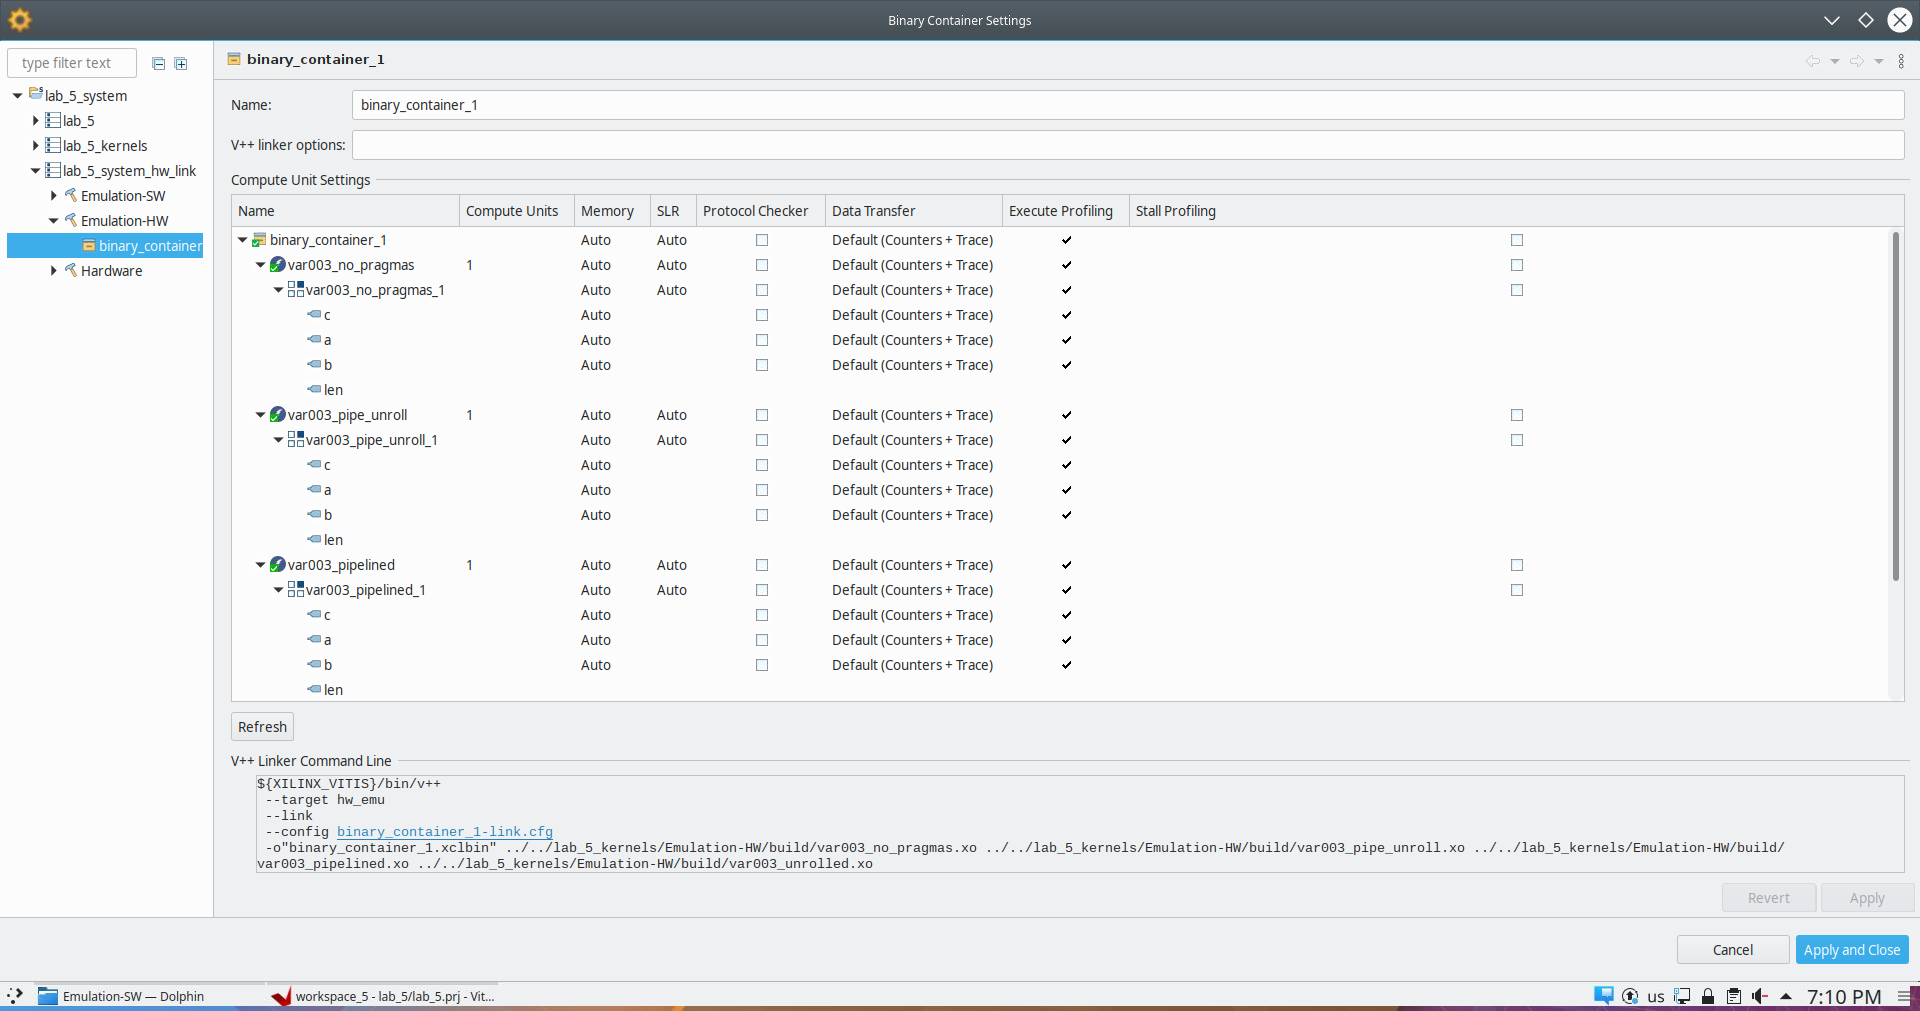
\includegraphics[width=0.9\linewidth]{img/hw-1}
	\caption{Assistant View}
	\label{fig:hw-1}
\end{figure}

\begin{figure}[ht]
	\centering
	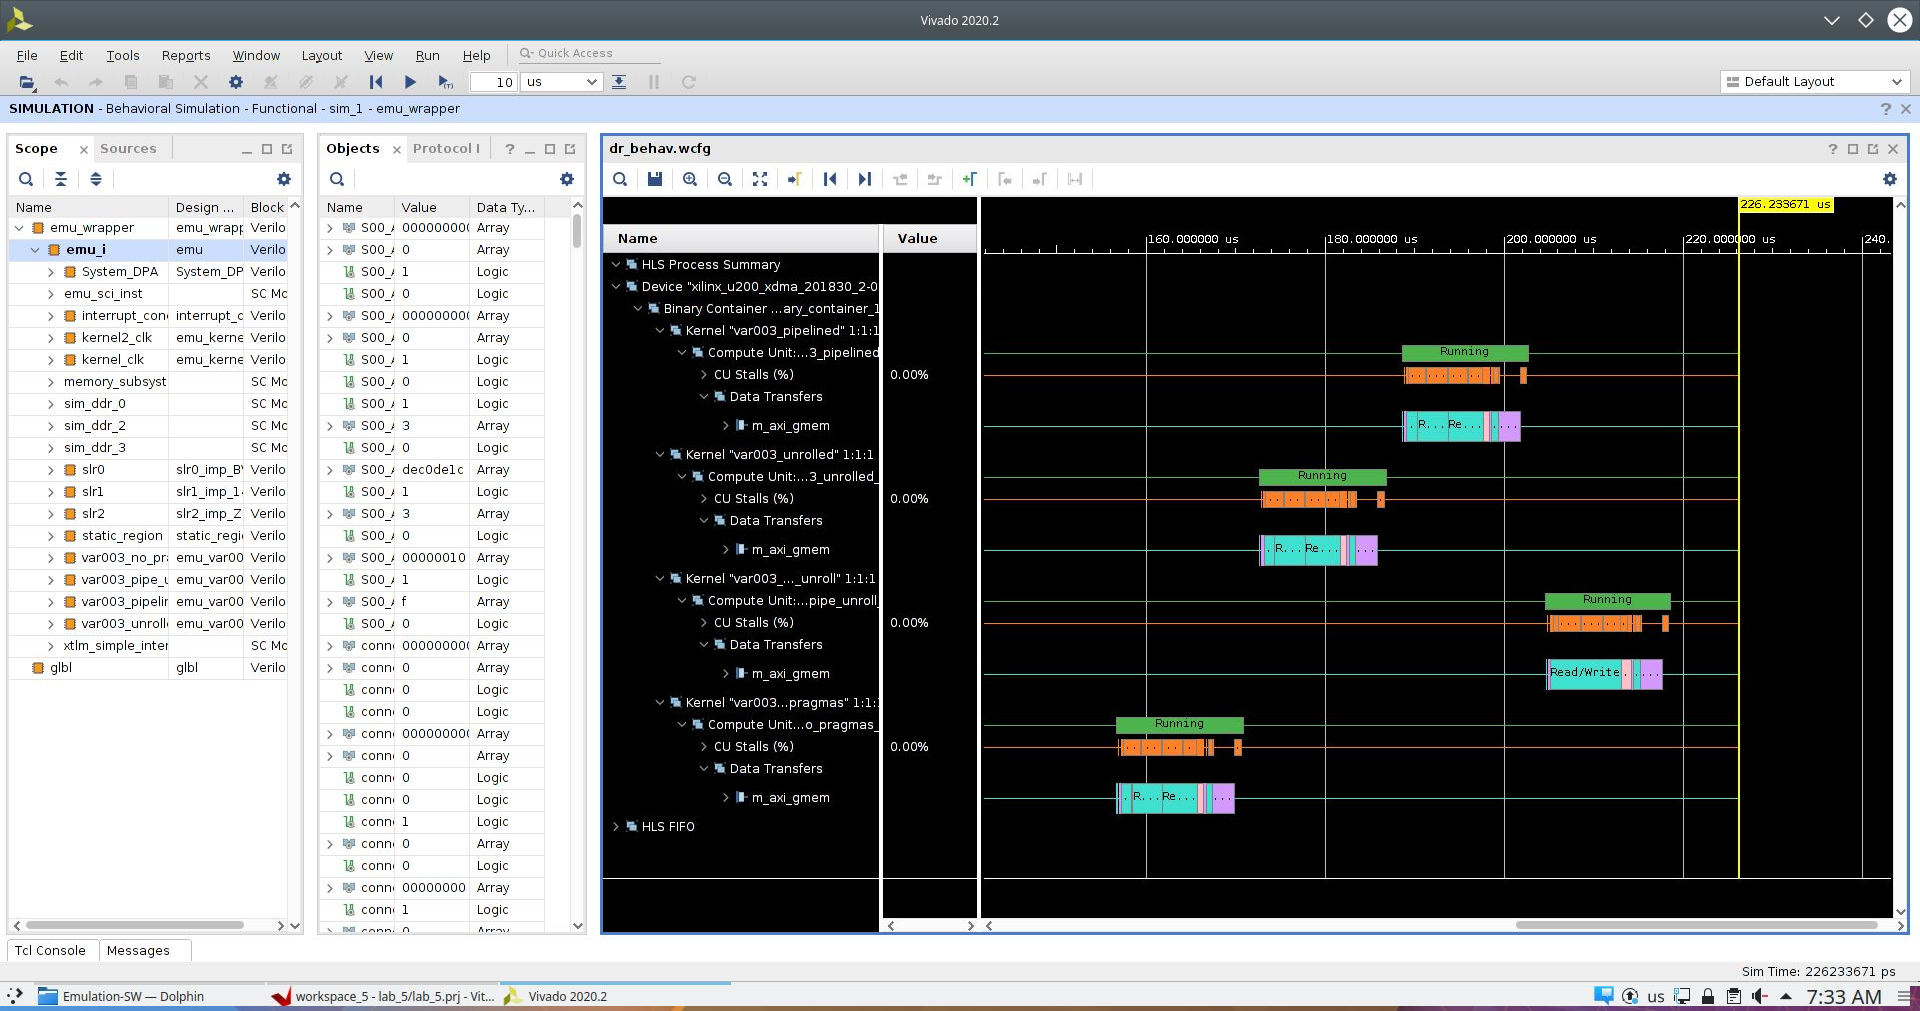
\includegraphics[width=0.9\linewidth]{img/hw-2}
	\caption{Окно внутрисхемного отладчика Vivado}
	\label{fig:hw-2}
\end{figure}

\chapter{Сборка и отладка проекта в режиме аппаратного
исполнения (Hardware)}

\begin{figure}[ht]
	\centering
	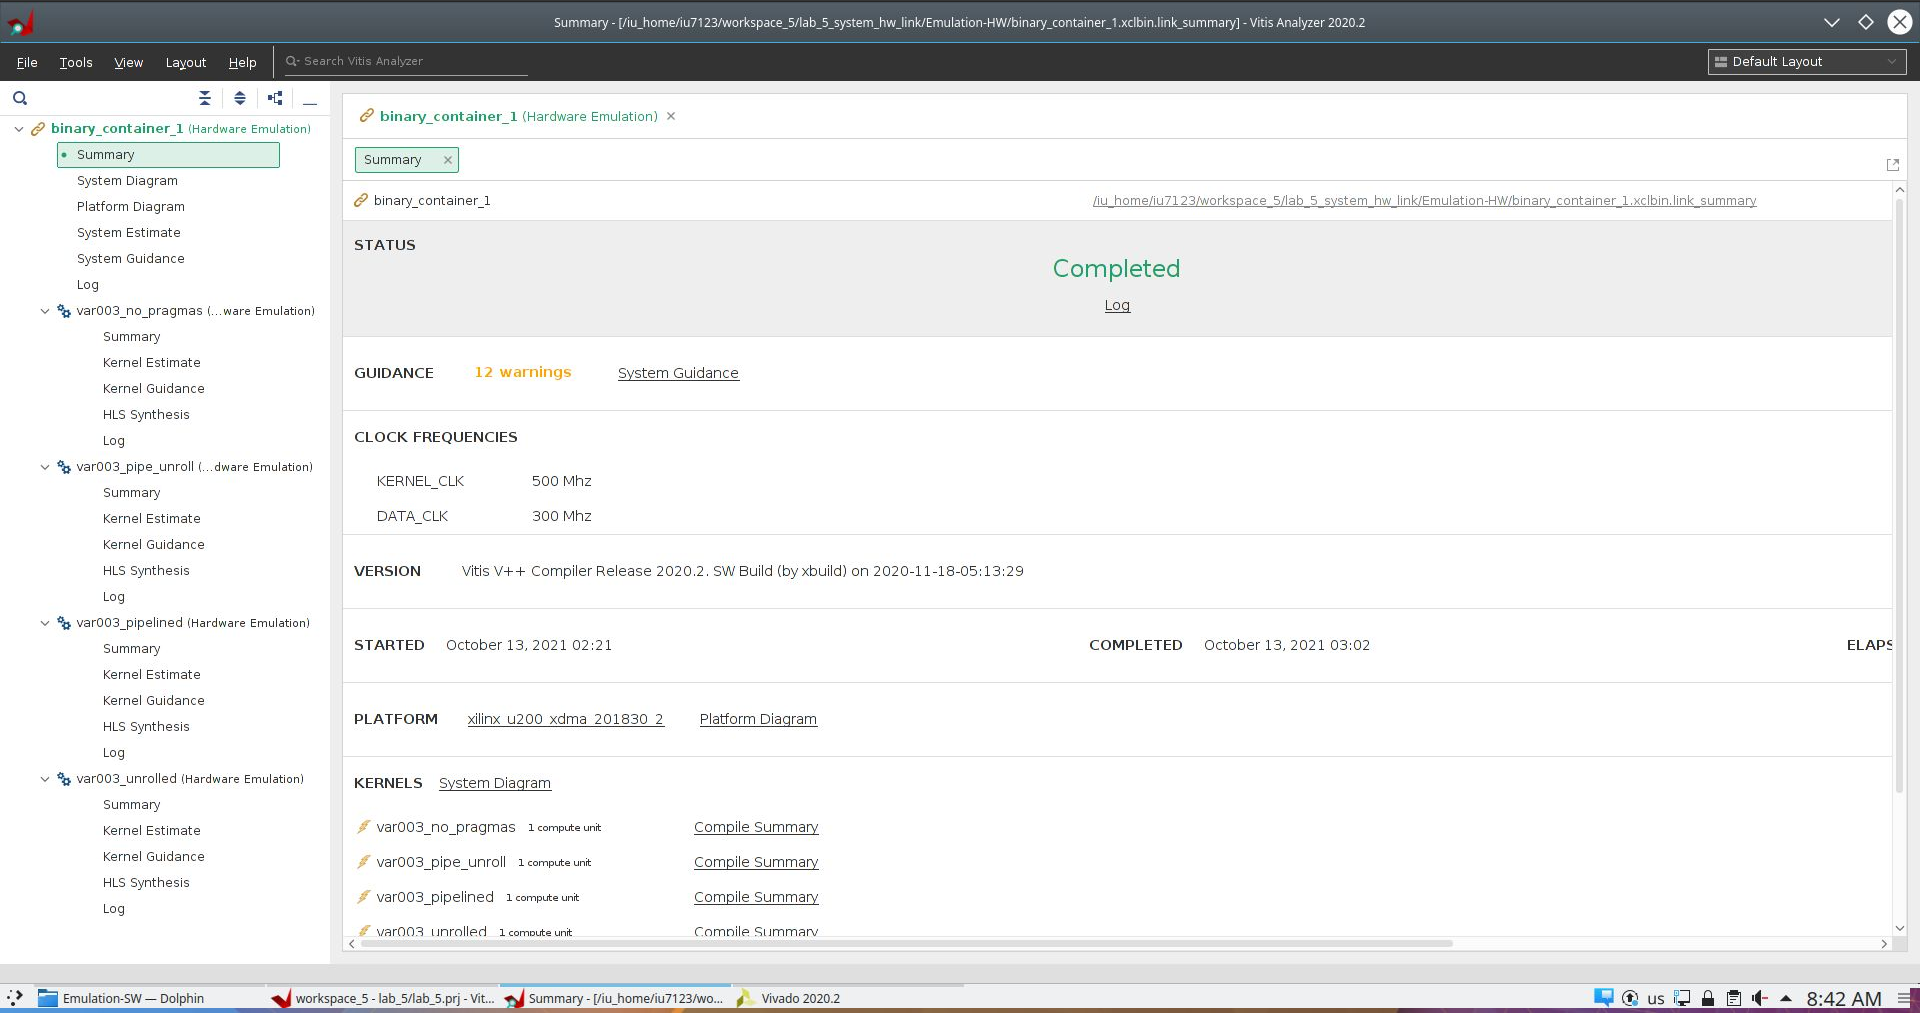
\includegraphics[width=0.9\linewidth]{img/hw-3}
	\caption{Содержимое вкладки Summary}
	\label{fig:hw-3}
\end{figure}

\begin{figure}[ht]
	\centering
	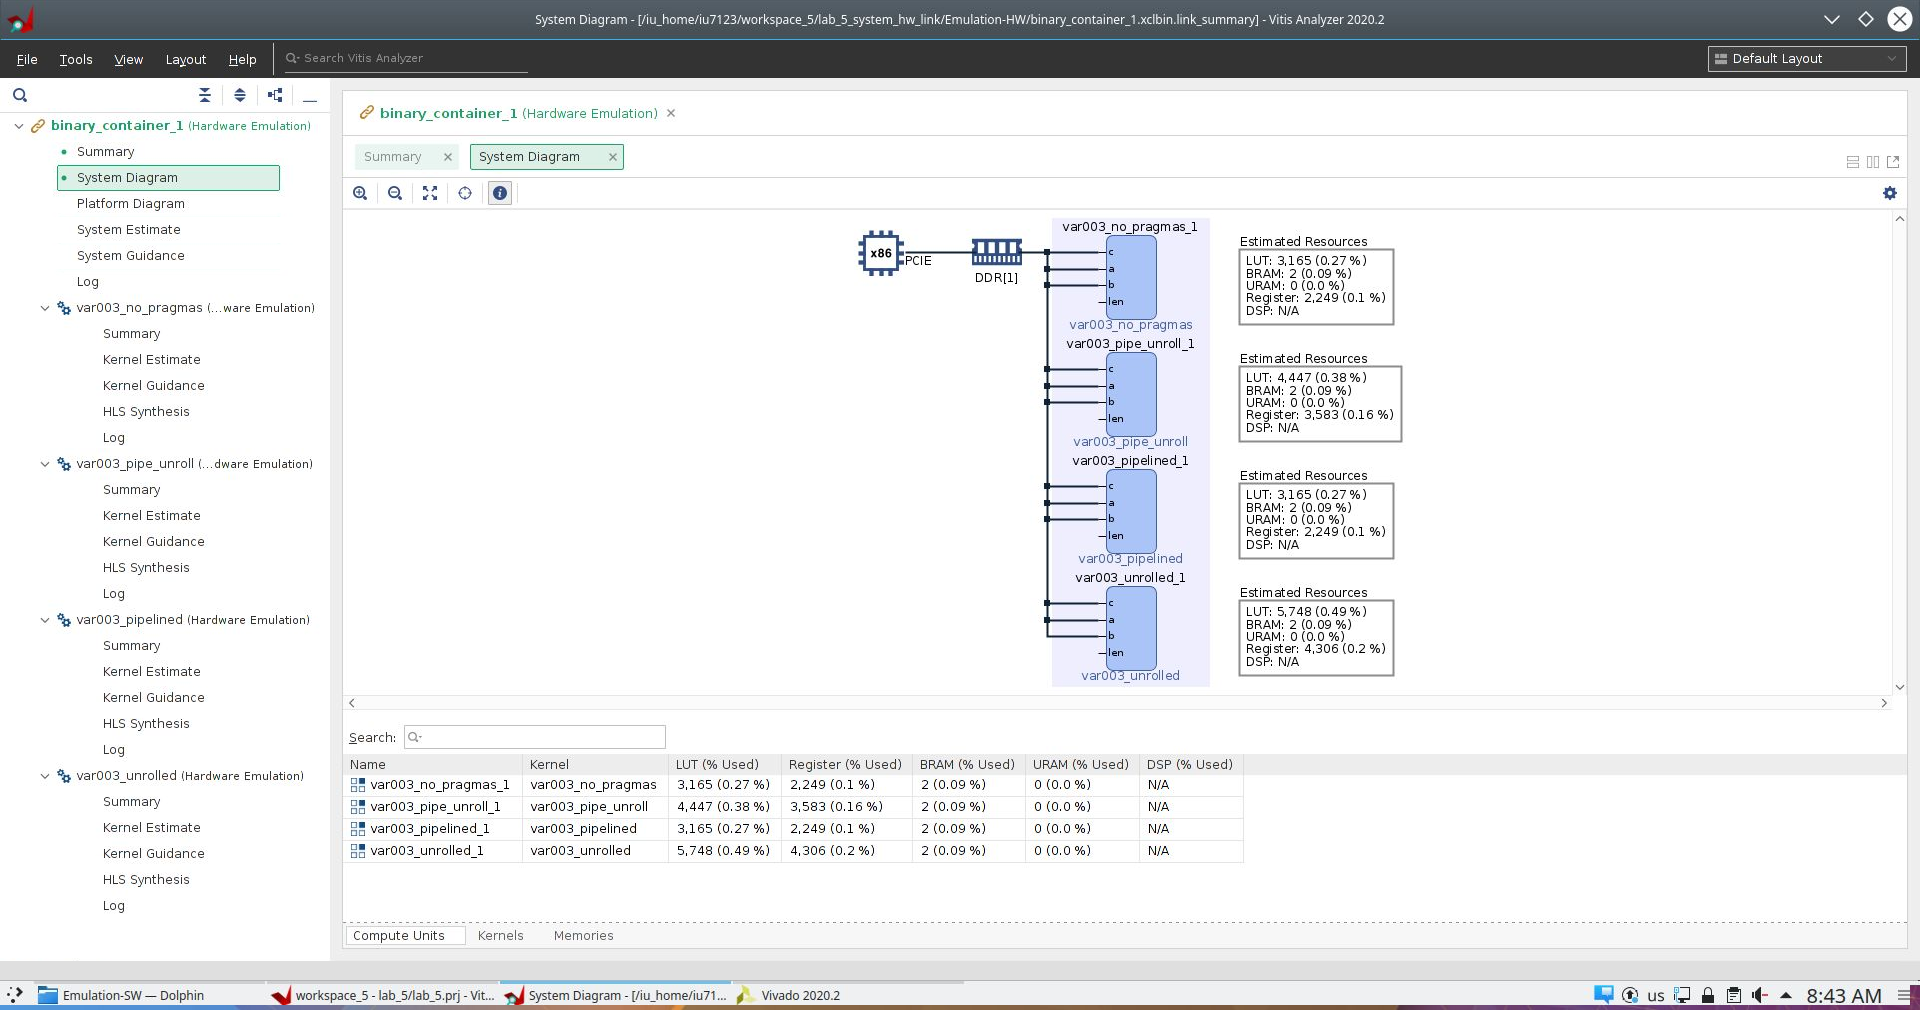
\includegraphics[width=0.9\linewidth]{img/hw-4}
	\caption{Содержимое вкладки System Diagram}
	\label{fig:hw-4}
\end{figure}

\begin{figure}[ht]
	\centering
	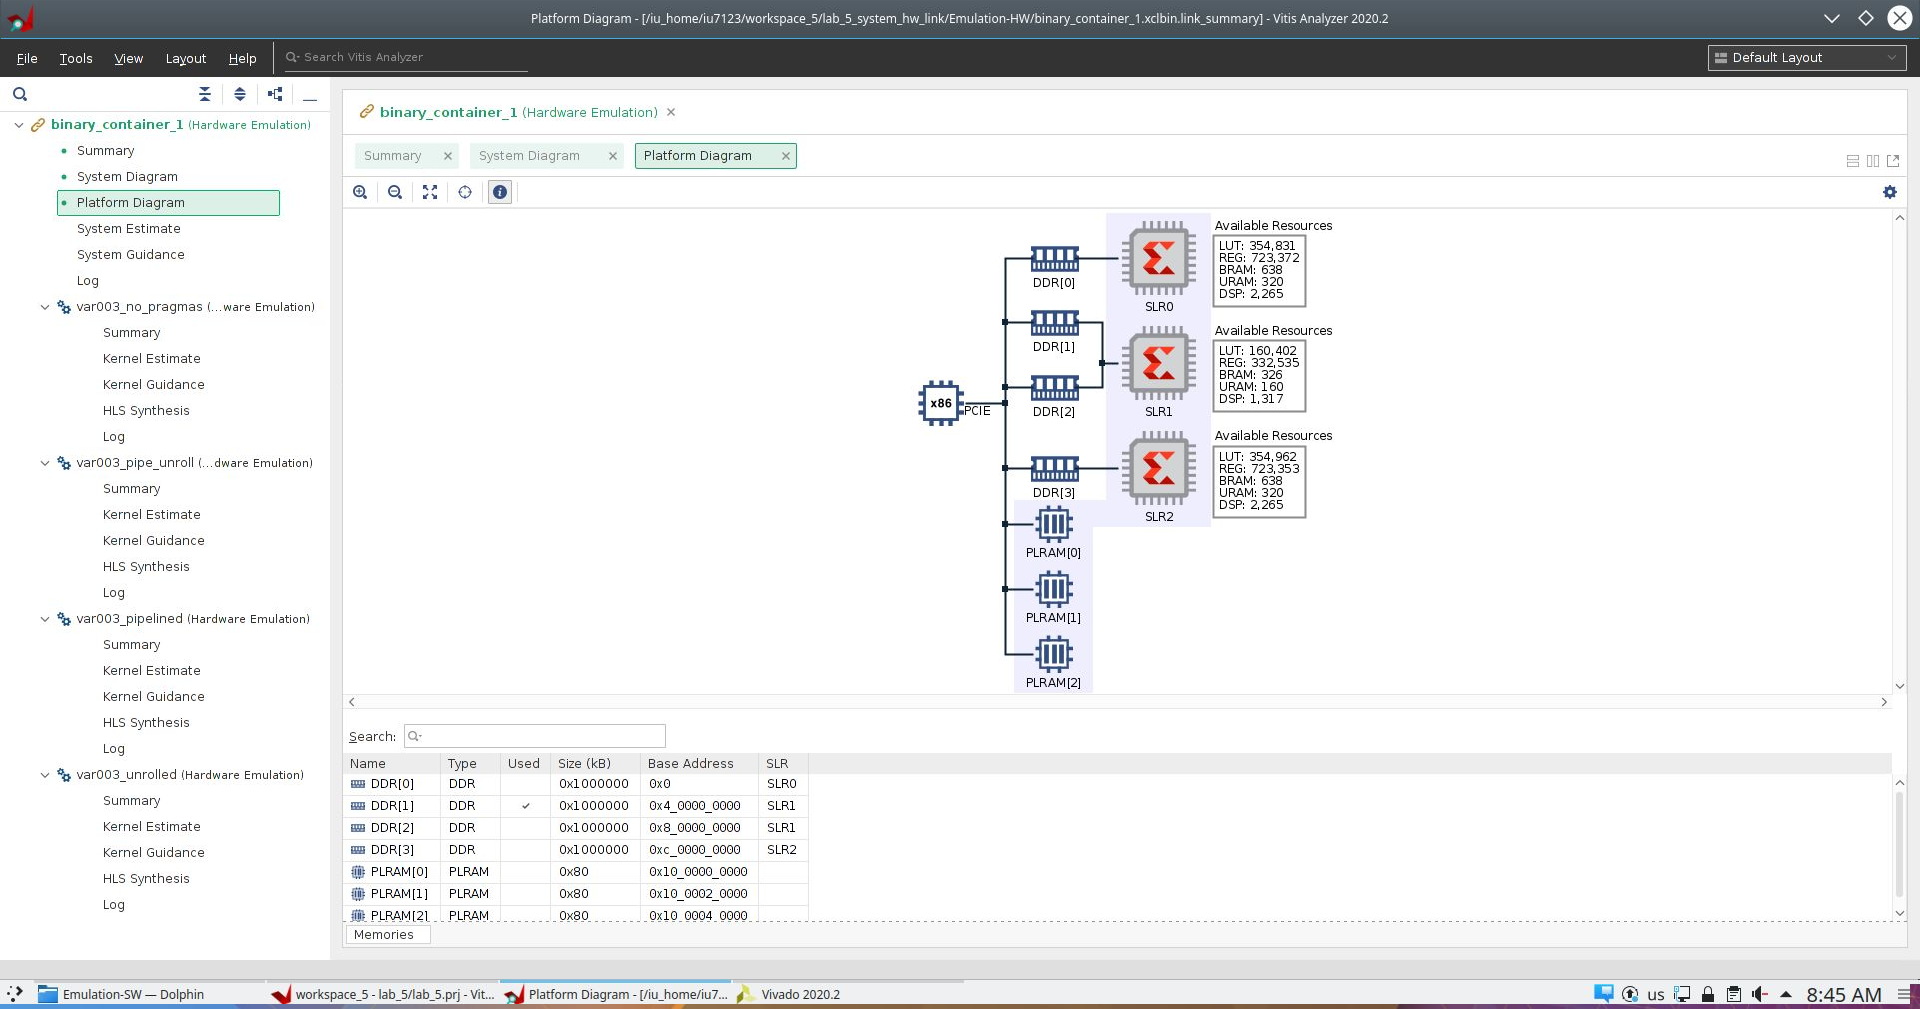
\includegraphics[width=0.9\linewidth]{img/hw-5}
	\caption{Содержимое вкладки Platform Diagram}
	\label{fig:hw-5}
\end{figure}

\begin{figure}[ht]
	\centering
	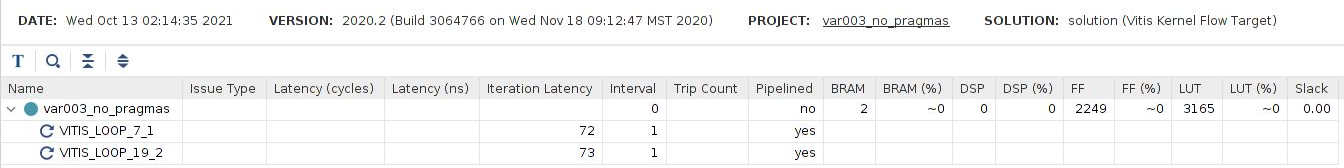
\includegraphics[width=0.9\linewidth]{img/hw-hls-1}
	\caption{HLS (1)}
	\label{fig:hw-hls-1}
\end{figure}

\begin{figure}[ht]
	\centering
	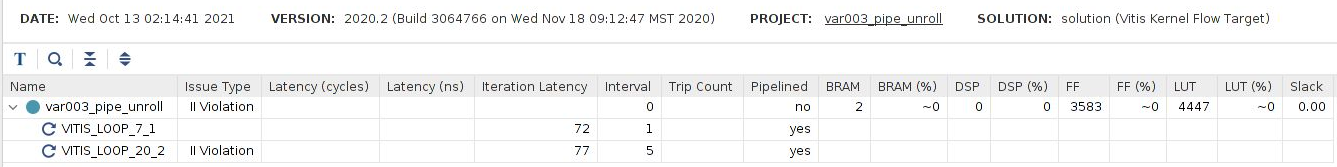
\includegraphics[width=0.9\linewidth]{img/hw-hls-2}
	\caption{HLS (2)}
	\label{fig:hw-hls-2}
\end{figure}

\begin{figure}[ht]
	\centering
	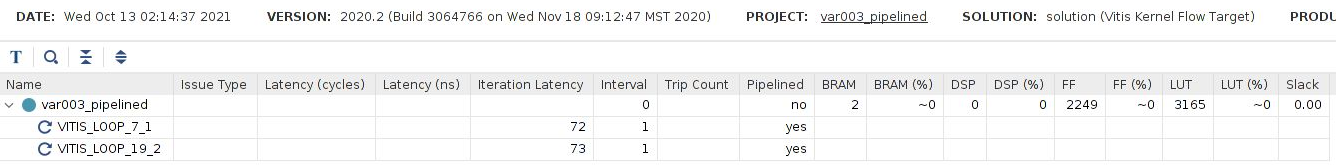
\includegraphics[width=0.9\linewidth]{img/hw-hls-3}
	\caption{HLS (3)}
	\label{fig:hw-hls-3}
\end{figure}

\begin{figure}[ht]
	\centering
	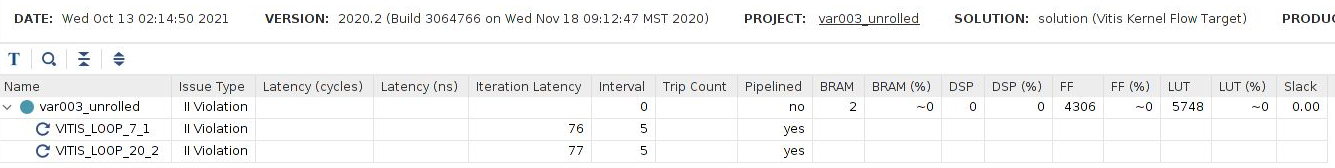
\includegraphics[width=0.9	\linewidth]{img/hw-hls-4}
	\caption{HLS (4)}
	\label{fig:hw-hls-4}
\end{figure}

\clearpage

\begin{lstlisting}[caption=Результаты работы]
Found Platform
Platform Name: Xilinx
INFO: Reading /iu_home/iu7123/workspace_5/lab_5_system/Hardware/binary_container_1.xclbin
Loading: '/iu_home/iu7123/workspace_5/lab_5_system/Hardware/binary_container_1.xclbin'
Trying to program device[0]: xilinx_u200_xdma_201830_2
Device[0]: program successful!
|-------------------------+-------------------------|
| Kernel                  |    Wall-Clock Time (ns) |
|-------------------------+-------------------------|
| var003_no_pragmas       |                 3077065 |
|-------------------------+-------------------------|
| var001_unrolled         |                 1029812 |
|-------------------------+-------------------------|
| var003_pipelined        |                  604712 |
|-------------------------+-------------------------|
| var003_pipe_unroll      |                  644299 |
|-------------------------+-------------------------|
Note: Wall Clock Time is meaningful for real hardware execution only, not for emulation.
Please refer to profile summary for kernel execution time for hardware emulation.
TEST PASSED.
\end{lstlisting}
